\section{Introduction}
\label{sec:intro}
\begin{figure}[t]
\centering
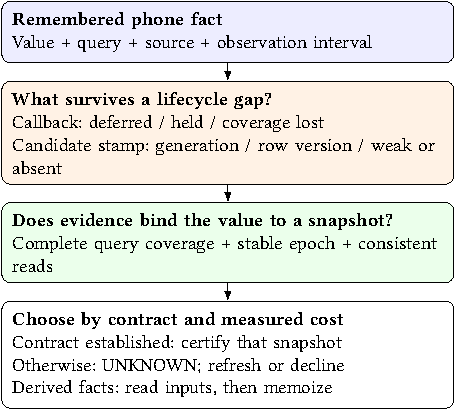
\includegraphics[width=\columnwidth]{figures/fig1-evidence-map.pdf}
\caption{The evidence map separates notification delivery, candidate stamps and snapshot certification. No branch certifies a later action automatically.}
\Description{Four linked boxes show a remembered fact, evidence surviving a lifecycle gap, the conditions for snapshot certification, and the choice between certification, UNKNOWN, refresh and memoization.}
\label{fig:overview}
\end{figure}

Mobile agents remember contacts, messages, photos and meetings across tasks. MobileGPT maintains app memory~\cite{lee2024mobilegpt}; broader memory systems persist facts for later reasoning~\cite{packer2023memgpt,chhikara2025mem0,rasmussen2025zep}. A remembered copy of phone state is a cache entry. Before using it, a client needs evidence that its query still has the same answer.

Android makes that evidence deployment-dependent. Processes can be killed, frozen or restarted~\cite{lebeck2020marvin,liang2020acclaim,android_freezer,android_doze}, and SMS, call-log and all-files access are restricted~\cite{play_smscalllog,play_allfiles}. Research agents often read through a host-side controller~\cite{rawles2025androidworld,zhang2025appagent,wang2024mobileagent}, whose on-device notification relay inherits Android's lifecycle and callback timing. We measure what such clients can infer for seven sources and four deployments, on Android~13 and 15 emulators and on rented Pixel~8 and Galaxy~S25 phones.

\paragraph{What the phones show.} Four results shape the design. (1) \emph{Stamps are candidates, not certificates.} Reading a value and then its version certified a changed value in \PhysRaceStale of \PhysRaceTrials races on the Pixel~8 and \PhysSamsungRaceStale of \PhysSamsungRaceTrials on the Galaxy~S25 (Tables~\ref{tab:phys-race} and~\ref{tab:phys-samsung}); a Contacts provider reset left the stamp unchanged in \PhysResetSameStamp Pixel~8 trials (\S\ref{sec:meas-gaps}). (2) \emph{The device decides the gap.} Pixel~8 units ran \PhysBuilds builds and \PhysFreezerOffTrialUnits had the cached-app freezer off by default; the Galaxy~S25 froze a cached client in \PhysSamsungFrozen attempts (Pixel~8: \PhysFreezerProbeFrozen); and its Contacts notifications carry a hidden no-delay flag, so a background client heard Contacts changes after \PhysSamsungBgMedian, against \PhysDeployBgMedian on the Pixel~8, while MediaStore stayed deferred (Table~\ref{tab:phys-samsung}). (3) \emph{Re-validation at the action boundary does not close the race:} on the Pixel~8, \PhysBndOverlapStale changes overlapping the check or the effect still produced stale effects (Table~\ref{tab:phys-boundary}). (4) \emph{Cheaper is not safer.} Through a host helper, batched optimistic stamp checks beat batched refresh only by re-reading fewer facts (from \PhysHostReadsStampMin to \PhysHostReadsStampMax against \PhysHostReadsRefresh; Table~\ref{tab:phys-host}); that is the policy of result (1), so we do not recommend it.

\paragraph{Gap classes.} A gap defers callbacks, holds them during freezing or loses observer coverage, and each class needs a different strategy: deferred or held callbacks leave event-only invalidation stale until delivery, while lost coverage makes persisted flags unsafe and requires refresh after restart. Timestamps are weaker evidence than versions, and file mtimes were coarse on the emulators but not on the Pixel~8.

\paragraph{Two policies.} \stamp is an optimistic diagnostic baseline that reads a value and then its stamp, so a write between those reads can label an old value with a new stamp. \sys instead requires a consistent observation, a complete validation interval and reset-safe evidence; stock adapters without that contract return \Unknown, and a cooperative transactional provider supplies positive controls.

\paragraph{Practical consequences.} Inside the client, direct provider refresh is faster than \stamp (\CostGl versus \CostLm\,ms per decision on the emulators, \PhysCostGl versus \PhysCostLm\,ms on the Pixel~8), and input memoization reduces model calls. A notification relay is cheaper still but inherits its helper's lifecycle. Because the gap class must be observed on the device, Table~\ref{tab:guidance} starts from a run-time check and then chooses by deployment, evidence and measured cost.

\paragraph{Contributions.} We provide (1) an Android source and deployment evidence map with lifecycle measurements on emulators and two rented phone models; (2) comparisons of notification, refresh, memoization and optimistic validation, with independent trial counts and matched host transport; and (3) a conditional consistency contract, device-executed counterexamples and a cooperative positive control. Version validation itself is established practice~\cite{gray1989leases,howard1988afs,rfc9110,rfc6578}. Our contribution is determining where its assumptions hold, fail or remain unestablished for this mobile workload.
